%! TeX program = xelatex

\documentclass[12pt, a4paper]{article}
\usepackage{cmap}
\usepackage[fontsize=12pt]{scrextend}
\usepackage[T2A]{fontenc}
\usepackage[utf8]{inputenc}
\usepackage[english,russian]{babel}
\usepackage{amsmath,amsfonts,amssymb,amsthm,mathtools}
\usepackage[left=20mm, top=20mm, right=20mm, bottom=20mm, nohead, footskip=1cm]{geometry}
\usepackage{multirow}
\usepackage{array}
\usepackage{multicol}
\usepackage{graphicx}
\usepackage{wrapfig}
\usepackage{indentfirst}
\usepackage{enumitem}

\usepackage{polyglossia}
\usepackage{titlesec}
\usepackage{sectsty}
\usepackage{setspace}
\usepackage{fontspec}
\defaultfontfeatures{Mapping=tex-text}

\usepackage{fancyvrb}
\fvset{tabsize=4}

\usepackage{lipsum}
\usepackage{tocloft}
\usepackage[dvipsnames]{xcolor}

\usepackage{caption}
%\captionsetup{labelfont=it, textfont=it}
%\captionsetup[figure]{name=Схема}

\usepackage{hyperref}

\hypersetup{
    colorlinks=false,
    linktoc=all
}
\urlstyle{same}

\setmainlanguage{english}
\setotherlanguage{russian}
\setkeys{russian}{babelshorthands=true}
\setmainfont{Times New Roman}
\newfontfamily\cyrillicfont{Times New Roman}
\setmonofont{FreeMono}
%\let\cyrillicfonttt\ttfamily
%\onehalfspacing

%\allsectionsfont{\centering}
\renewcommand{\cftsecleader}{\cftdotfill{\cftdotsep}}

%======================================SECTIONING=========================================
%\makeatletter
%\renewcommand*\l@section{\@dottedtocline{1}{1.5em}{2.3em}}
%\makeatother
%======================================SECTIONING=========================================

\pretolerance=6000
\tolerance=3000
\emergencystretch=4pt

\setlength\intextsep{10pt}

\graphicspath{{./visuals/}}
\setlength{\parskip}{0.3125cm}
\setlength{\parindent}{1.25cm}
\setlength{\columnsep}{1cm}
\author{Grigoryev Mikhail}
\title{Algs lab}

\begin{document}

\thispagestyle{empty}

\vspace{30mm}

\begin{center}
FEDERAL STATE AUTONOMOUS EDUCATIONAL INSTITUTION \\
OF HIGHER EDUCATION \\
ITMO UNIVERSITY

\vspace{40mm}

{\large \textbf{Report \\
on the practical task No. 8 \\
"Practical analysis of advanced algorithms."}}
\end{center}

\vspace{15mm}

\begin{flushright}
{\large Performed by \\
\textit{Mikhail Grigoryev (370852) \\
Semenova Valeria (370061) \\
Academic group J4133c \\}
Accepted by \\
Dr Petr Chunaev}
\end{flushright}

\vspace{80mm}

\begin{center}
St. Petersburg \\
2022
\end{center}

\newpage

\section*{Goal}
\addcontentsline{toc}{section}{Goal}

Practical analysis of advanced algorithms.

\section*{Formulation of the problem}
\addcontentsline{toc}{section}{Formulation of the problem}

Choose two algorithms not considered in the course from the selected sections of the book \textit{Introduction to algorithms} by \textit{Thomas H. Cormen et. al.}, implement them and produce experiments on them considering their time and space complexity. Analyze the results of experiments as well as theoretical foundations of the algorithms.

\section*{Brief theoretical part}
\addcontentsline{toc}{section}{Brief theoretical part}

The two chosen algorithms from the chapter \textit{Minimum Spanning Trees} were Kruskal's and Prim's algorithms of finding Minimum Spanning Trees of undirected weighted graphs.

\textbf{Minimum Spanning Tree} is a acyclic subset of a chosen graph that contains all its vertices and the edges with the minimum total weight (if graph is unweighted this means minimum number of edges). All algorithms for growing/finding MST are essentially loops adding safe edges to the growing tree (here pseudocode will be written in pythonic style):
\begin{Verbatim}
def mst(G, w):
	A = set()
	while (A does not form an ST):
		find an edge (u,v) that is safe for A
		A.add((u,v))
	return A
\end{Verbatim}

Then there is the question of finding the safe edge \texttt{(u,v)}. The rule for recognizing safe edges is formulated as follows:
\begin{quote}
	Let $G = (V,E)$ be a connected, undirected graph with a real-valued weight function $w$ defined on $E$. Let $A$ be a subset of $E$ that is included in some minimum spanning tree for $G$, let $(S, V-S)$ be any \textbf{cut} of $G$ that \textbf{respects} $A$, and let $(u,v)$ be a \textbf{light} edge \textbf{crossing} $(S, V-S)$. Then, edge $(u,v)$ is safe for $A$.
\end{quote}
In the thorem, several terms were used:
\begin{itemize}
	\item A \textbf{cut} is a partition of $V$ into two groups of vertices: $S$ and $V-S$.
	\item An edge $(u,v)$ \textbf{crosses} the cut if $u$ is in one partition and $v$ is in the other.
	\item If both $u$ and $v$ are in the same partition, the edge $(u,v)$ \textbf{respects} the cut.
	\item An edge crossing the cut is \textbf{light} if it has the least weight of all edges crossing this cut.
\end{itemize}

\newpage

In \textbf{Kruskal's algorithm} the set $A$ is a forest whose vertices are all the vertices of the initial graph. The safe edge is always a least-weighted edge that connects two distinct components of $A$. The algorithm looks like:
\begin{Verbatim}
def mst_kruskal(G, w):
	A = set()
	for vertex in G.V:
		make_set(vertex)
	
	sorted_edges = G.E.sort(lambda edge: edge['weight'])
	
	for edge in sorted_edges:
		u, v = edge[0], edge[1]
		if find_set(u) != find_set(v):
			A.add((u,v))
			union(u, v)
	
	return A
\end{Verbatim}
In the listing above there are three utility functions:
\begin{itemize}
	\item \texttt{make\_set(vertex)} -- function that makes a single-vertex tree out of vertex and stores it in some local variable (e.g. \texttt{trees});
	\item \texttt{find\_set(vertex)} -- function that finds a tree in \texttt{trees} that contains \texttt{vertex}.
	\item \texttt{union(vertex\_1, vertex\_2)} -- function that combines two trees containing \texttt{vertex\_1} and \texttt{vertex\_2} into one tree and stores it in the variable \texttt{trees} deleting the initial two trees.
\end{itemize}

\begin{wrapfigure}{r}{0.5\textwidth}
\centering
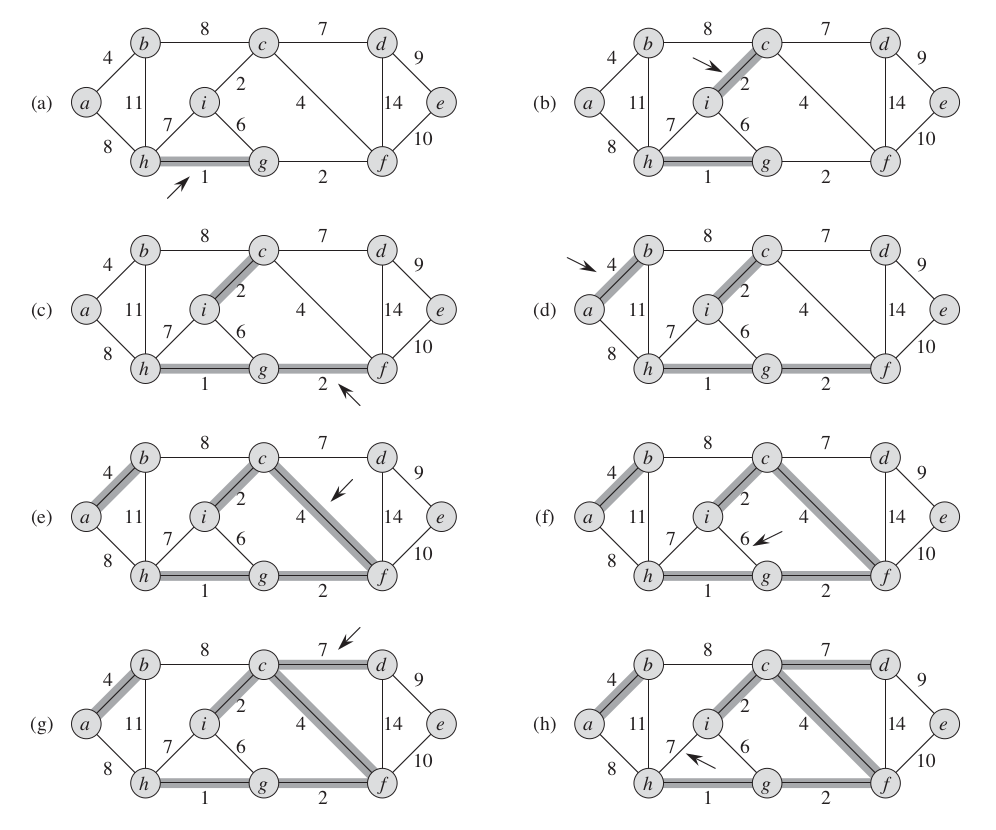
\includegraphics[width=0.49\textwidth]{kruskal.png}
\caption{The execution of Kruskal's algorithm (taken from the book \textit{Introduction to algorithms} by \textit{Thomas H. Cormen et. al.}).}
\end{wrapfigure}

Thus, the algorithm sorts all edges by weight. Then, at each iteration it takes the lightest edge and considers if it connects two trees in $A$ (to start, every vertex of $G = (V,E)$ is a tree in $A$). Sorting the edges takes $O(E \log E)$. The number of iterations is $E$. Each iteration two \texttt{find\_set(vertex)} and at most one \texttt{union(vertex\_1, vertex\_2)} are called (those operations on disjoint-set forest take $O(E \log V)$). In total, we have $O(2E \log (E \cdot V))$. As $E < V^2$, $\log E = O(\log V)$. Thus, total time complexity is $O(E \log V)$.

Space complexity of $O(V+E)$ is observed, as to keep track of all the vertices in the beginning and the respective subsets we need $O(V)$ and for all valid sorted edges to be included in the final MST we need $O(E)$.

\newpage

In \textbf{Prim's algorithm} the set $A$ is a single tree. The safe edge connects the tree to a vertex not in the tree as opposed to Kruskal's. It operates like Dijkstra's algorithm for finding the shortest path. The set $A$ is maintained as:
\[ A = \big\{ (v, v.parent) : \quad v \in V - \{ r \} - Q \big\}, \]\
where $r$ is the root of the Spanning Tree, $Q$ is the min-priority queue based on a \texttt{key} attribute (minimum weight of any edge connected to that vertex, if none, then $\infty$). Attribute $v.parent$ names the parent of $v$ in tree.
The algorithm looks like:
\begin{Verbatim}
def mst_prim(G, w, r):
	for u in G.V:
		u.key = infinity
		u.parent = None
	r.key = 0

	Q = G.V
	while len(Q) > 0:
		u = extract_min(Q)
		for v in G.adj[u]:
			if v in Q and w(u,v) < v.key:
				v.parent = u
				v.key = w(u,v)
\end{Verbatim}
In the listing above:
\begin{itemize}
	\item \texttt{extract\_min(Q)} -- function that extracts the minimally-weighted edge of the priority queue;
	\item \texttt{G.adj[u]} lists all neighbors of vertex \texttt{u}.
\end{itemize}

\begin{wrapfigure}{r}{0.5\textwidth}
\centering
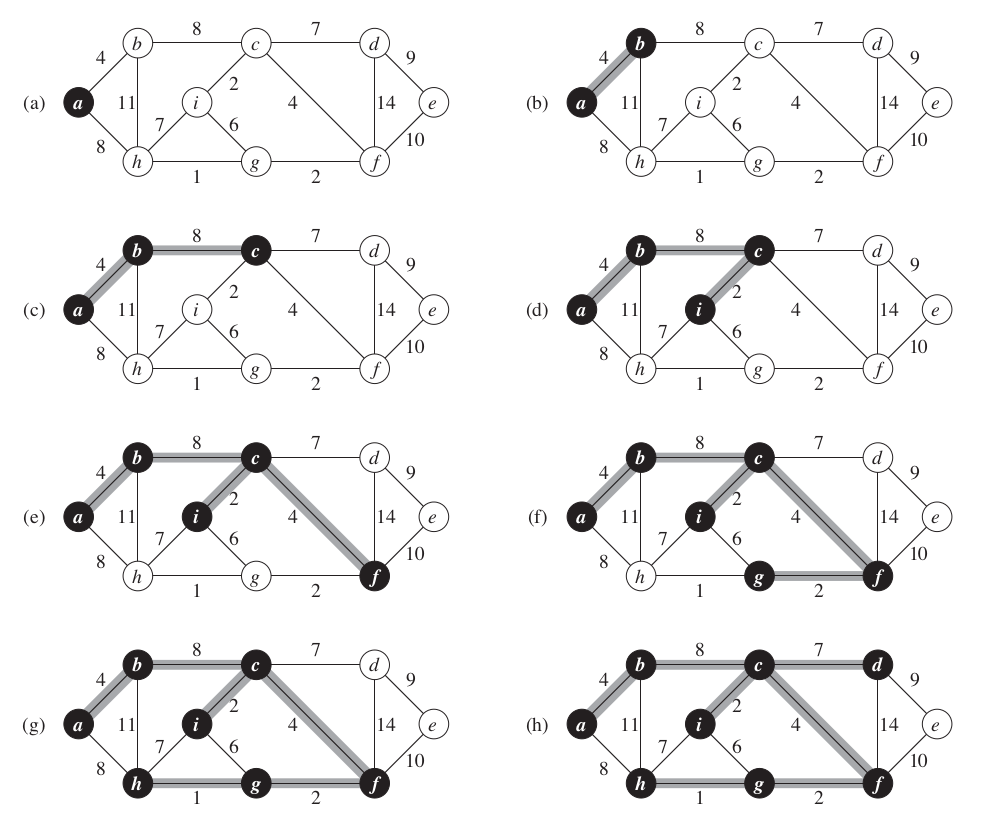
\includegraphics[width=0.49\textwidth]{prim.png}
\caption{The execution of Prim's algorithm (taken from the book \textit{Introduction to algorithms} by \textit{Thomas H. Cormen et. al.}).}
\end{wrapfigure}

Thus, the algorithm adds all vertices to a priority queue and then starts growing a tree from vertex \texttt{r}. In the while loop the algorithm takes first the lightest edge connected to the root (as all other keys are $\infty$) and in further iterations to any vertices in the tree. This lightest edge's end vertex is added to the tree and its neighbors' keys and parent are recalculated. Time complexity depends on the implementation of \texttt{Q}. In case of NetworkX, it is a binary min-heap. While loop executes $V$ times (all vertices in priority queue) and \texttt{extract\_min} (the longest running function within the loop) takes $O( \log V )$ in case of binary heap. The for loop within the while loop runs $O(E)$ times in total as the sum of the lengths of all adjacency lists is $|E|$. The last line implicitly calls \texttt{decrease\_key} in a binary heap which runs in $O( \log V )$. Total time complexity is $O( V \log V + E \log V ) = O(E \log V)$, which is the same as Kruskal's.

Space complexity is $O(V+E)$ for the same reason as Kruskal's.

\newpage

\section*{Results}
\addcontentsline{toc}{section}{Results}

Both algorithms were implemented from the NetworkX library. Graphs of varying $V$ and $E$ were generated using the same library. Runtimes of both algorithms were measured as an average of 3 (each time new graph) so as to break the dependency of the runtime on the produced random graph and OS processes. The results were plotted in 3D as a function $T = f(V, E)$.

The theoretical time complexity function with additional constants $a$, $b$, $c$ and $d$:
\[ T = a + b \cdot E \cdot \log_2 (c \cdot V + d) \]
was fit onto the experimental data. For the results from random graphs (stored in the repository as kruskal.npz and prim.npz) those constants were written to the table below.
\begin{center}
\begin{tabular}{ccc}
	\hline
	algorithm & & function w/constants \\ \hline
	Kruskal's & & $T = 0.0149 + 0.000065 \cdot E \cdot \log_2 (0.0041 \cdot V + 0.9935)$ \\
	Prim's    & & $T = 0.0130 + 0.000047 \cdot E \cdot \log_2 (0.0072 \cdot V + 0.9503)$ \\ \hline
\end{tabular}
\end{center}

\begin{figure}[!h]
\centering
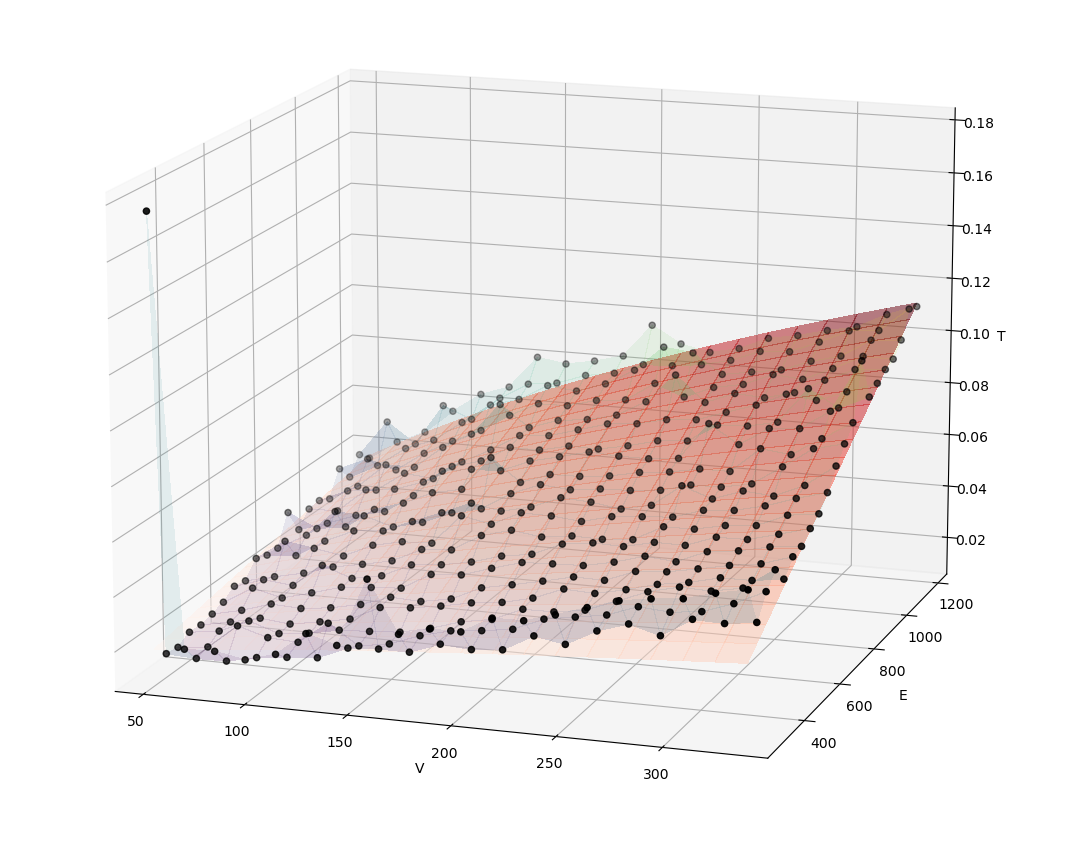
\includegraphics[width=0.45\textwidth]{kruskal_1.png}
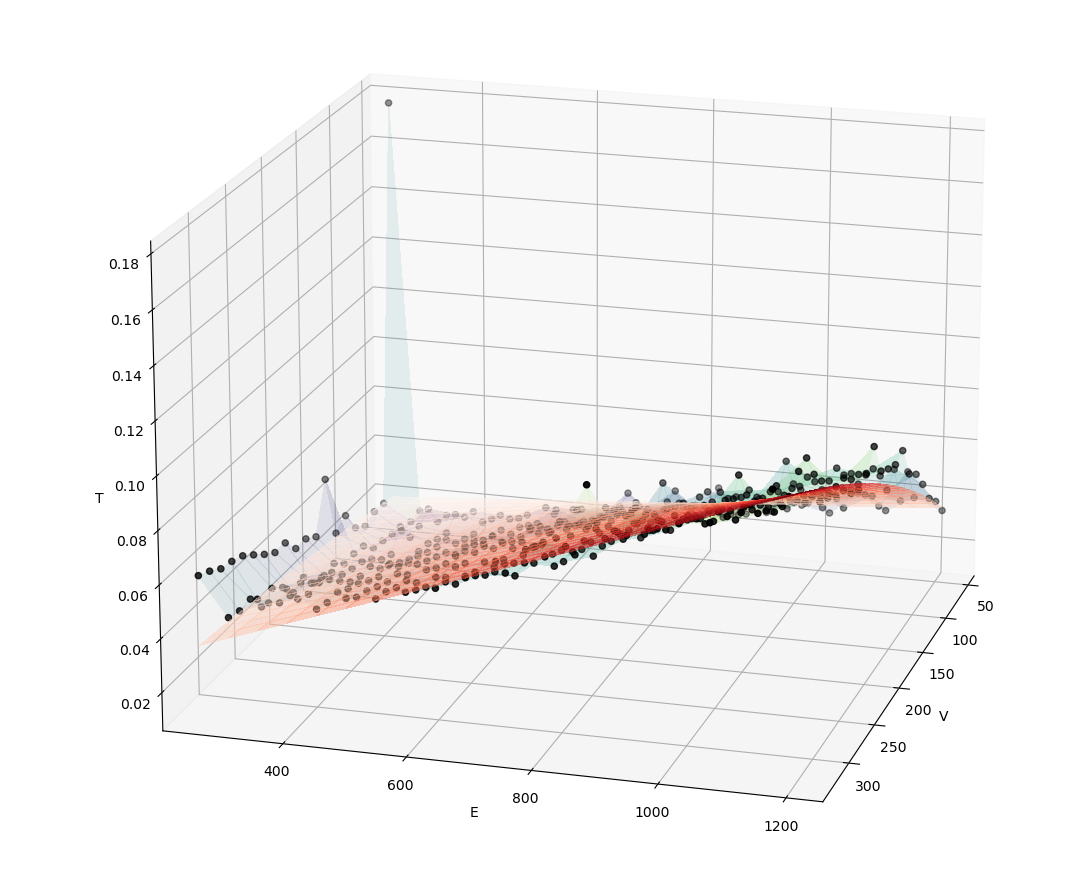
\includegraphics[width=0.45\textwidth]{kruskal_2.png}
\caption{Theoretical time complexity surface fitted on experimental runtimes for Kruskal's algorithm.}
\end{figure}

\begin{figure}[!h]
\centering
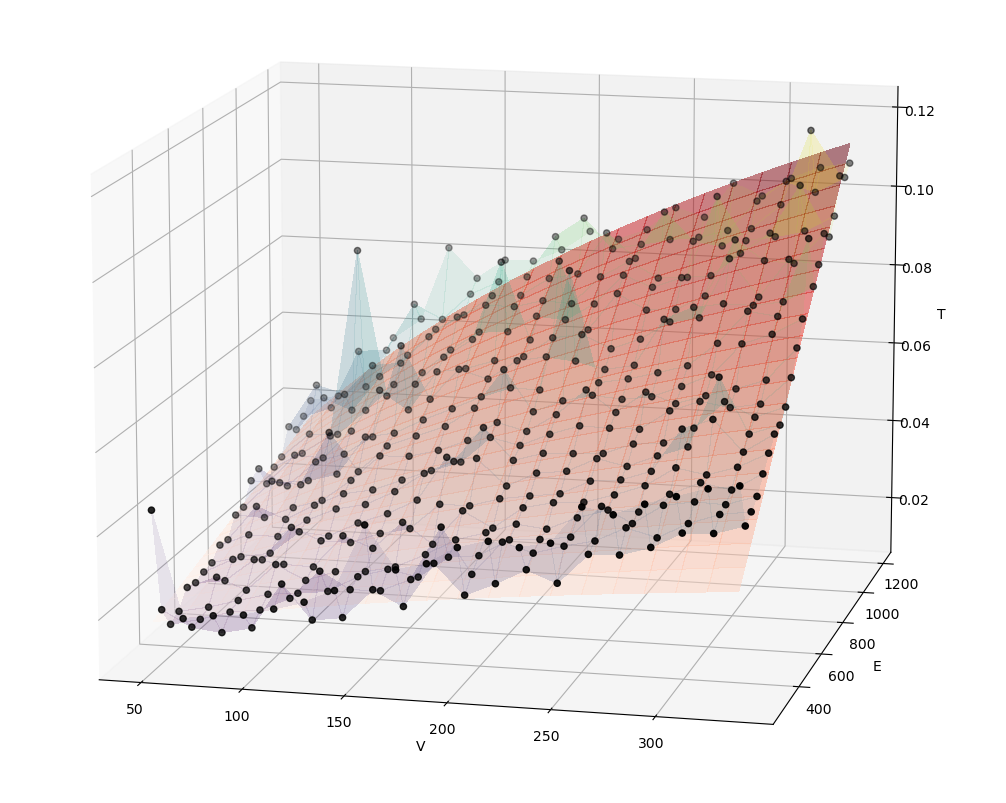
\includegraphics[width=0.45\textwidth]{prim_1.png}
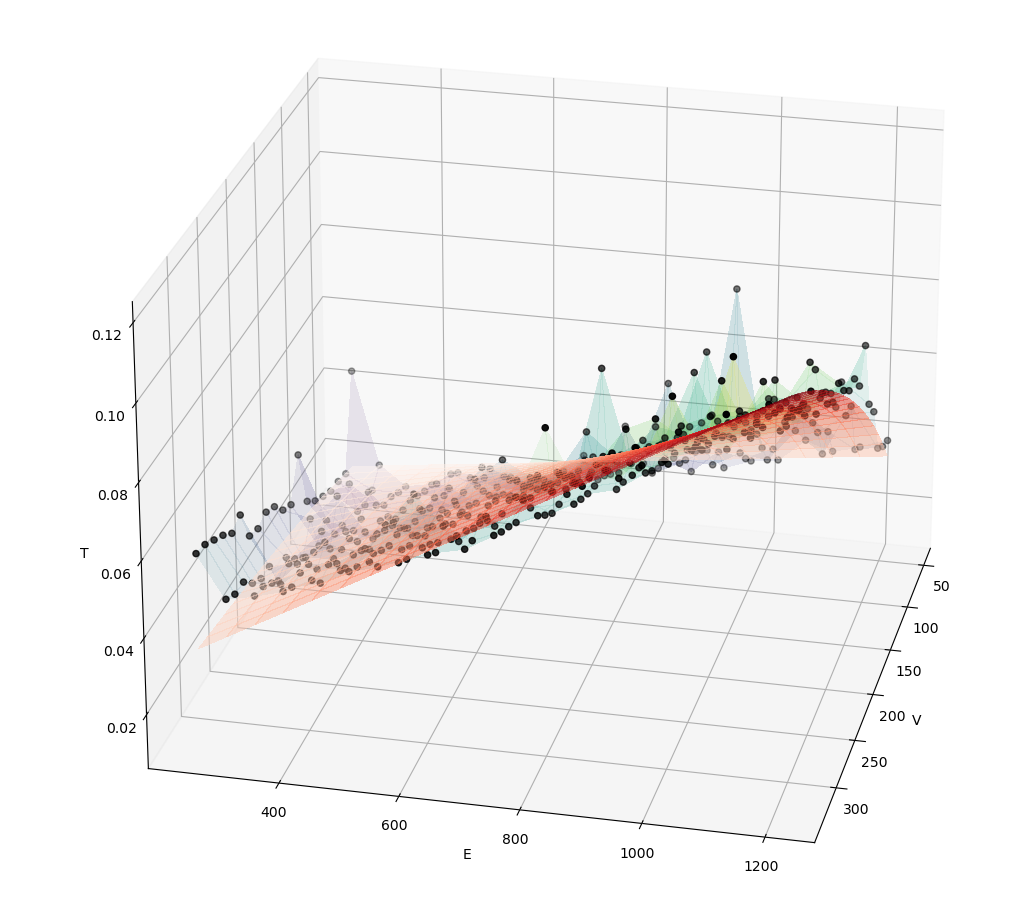
\includegraphics[width=0.45\textwidth]{prim_2.png}
\caption{Theoretical time complexity surface fitted on experimental runtimes for Prim's algorithm.}
\end{figure}

\noindent
The theoretical time complexities were fitted successfully thus proving their correctness.

\newpage

\section*{Conclusions}
\addcontentsline{toc}{section}{Conclusions}

Kruskal's and Prim's algorithms of finding the Minimum Spanning Tree of a weighted graph were analyzed theoretically and tested in terms of runtime of graphs of varying $V$ and $E$. The results were plotted in 3D and theoretical time complexities were successfully fitted onto the experimental data.

\section*{Appendix}
\addcontentsline{toc}{section}{Appendix}

GitHub link: \url{https://github.com/Dormant512/itmo_lab_listings/blob/main/lab8.py}.

\begin{figure}[!h]
\centering

\includegraphics[width=0.25\textwidth]{lab8.png}
\end{figure}


\end{document}
